\chapter{Introduction}
\label{Chapter:Introduction}

Social media has been a rapidly growing industry in the 21st century, with the social network Facebook, one of the most prominent social media sites, worth just under \$315 billion dollars as of May 2016 despite only being founded in 2004 \cite{Forbes:Facebook}. However, with the popularity of Facebook and other social networks such as Twitter and Instagram, numerous social issues have arisen which are yet to be fully addressed. Fidelis is an alternative to these networks, which attempts to address these issues. This report provides an overview of the requirements of the social network Fidelis, as well as the strategies used to design, develop and then test the system and a review of what this project has achieved.

\section{Problem Statement}
\label{Section:ProblemStatement}
Social networking platforms are now a well established part of day-to-day life for many people. These platforms are used around the world by a vast number of individuals. Figure \ref{fig:SocialMediaRegionGender} gives some insight into the use of social media around the world. With such a large number of users spending large amounts of time using these platforms, it is clear that they have a significant influence on modern life.

\begin{figure}[H]
  \centering
  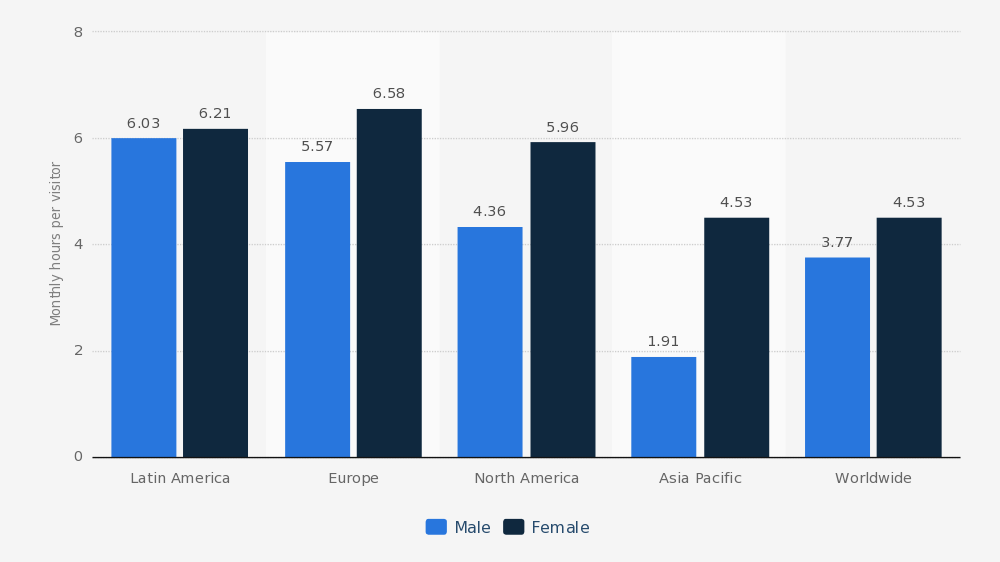
\includegraphics[width=0.75\textwidth]{Images/Introduction/SocialMediaRegionGender}
  \caption{User engagement June 2015, by region and gender \cite{Statista:SocialMediaRegionGender}} \label{fig:SocialMediaRegionGender} 
\end{figure}

Many existing platforms, of course, aim to provide the best possible user experience, however there are still some areas that can be improved upon. For example, Figure \ref{fig:TrollingByTopic} shows a number of topics on which respondents had witnessed internet `trolling' in a 2014 survey. This data demonstrates the prevalence of online abuse, with 65\% of those questioned responding that they have witnessed it in some form. Fidelis is designed to combat these kinds of issues by using a range of techniques to create a trust-centric social network.

\begin{figure}[H]
  \centering
  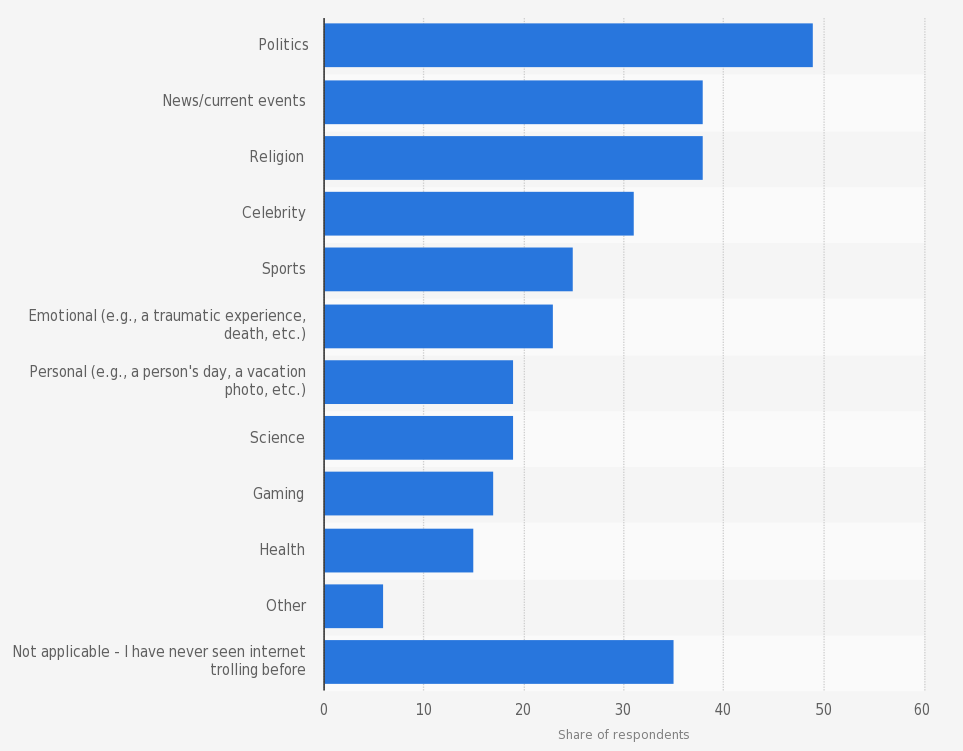
\includegraphics[width=0.75\textwidth]{Images/Introduction/TrollingByTopic}
  \caption{Internet trolling: topics online in the U.S. in 2014 \cite{Statista:TrollingByTopic}} \label{fig:TrollingByTopic} 
\end{figure}

\section{Project Aims}
Abuse detection, provision of user-specific content and reputation scoring are three key features which can be implemented to ensure that a social network is trustworthy. Therefore, the aim of this project is to build a new social network, Fidelis, which will demonstrate the methods of implementing these features and to evaluate how effective these methods are in solving the issues which established social networks currently face in their attempt to earn and retain the trust of their users.

\section{Project Motivation}
As mentioned in Section \ref{Section:ProblemStatement}, the popular social networks of today have given rise to numerous social issues. One of these issues is `trolling', with `The Guardian' reporting that ``one in four teenagers suffered hate incidents online last year'' \cite{Gani:Trolling}. In addition, there is an issue with the `echo chamber' effect, whereby ``users of the social media site interact most with those who share their political views'' \cite{Jackson:EchoChamber}. Facebook in particular have been accused of not doing enough to prevent this echo chamber effect, with former Times editor and News International chief executive Robert Thomson allegedly stating that Facebook ``not only help to promote `fake news', but will also reduce the diversity of opinion'' as a result of them ``routinely and selectively `unpublishing' certain views and news'' \cite{Orlowski:EchoChamber}. This causes a distortion between the ideas perceived on social media and opinions in the real world.

Social networks' current failure to find an effective solution to these pitfalls therefore offers the question, ``Can a network be created, that tailors the content users see based on what they would prefer to see?'' This does not only include filtering any abusive posts, but also offering them diverse content that is of interest to them, either based on the theme of the content or who posted it. By providing content based on the topics a user is interested in, even if that content offers an opposing viewpoint to the user's, the echo chamber effects should also be reduced, which will help create a more open discussion amongst users.

Since beginning this project, Twitter have made further efforts to reduce the amount of abuse which appears on their platform. This includes identifying accounts as they’re engaging in abusive behaviour, even if this behaviour hasn’t been reported and collapsing potentially abusive or low-quality Tweets \cite{Twitter:Safety}, both of which are features being implemented as a part of this project. With Twitter taking steps to make their site safer by implementing similar features to Fidelis highlights the relevance of such a project at this current time.

\section{Project Stakeholders}
The internal stakeholders for this project are the development team - Isheanesu Gambe, Naqash Tanzeel, Thomas Mcaloone and Jordan Olney - and Dr Matthew Leeke, who is the project supervisor. To ensure the project is successful, the wider public will also be involved to offer feedback on the progress of Fidelis throughout the duration of the project. In order to avoid a cold start, data from other social networks will be required to provide Fidelis with realistic posts, which can be used to train machine learning models. Therefore, the Twitter accounts of multiple stakeholders, both external and internal, will be used, so that large quantities of data can be collected in a short period of time, without exceeding the rate limits imposed by the Twitter API.

\section{Report Structure}
The purpose of this report is to provide a comprehensive account of the process undertaken whilst developing the system associated with the project. The report can been broken down into 3 main sections which identify the high level stages this project went through, which are:

\paragraph{Research and Analysis}
An introduction to the problem being faced and combated, motivations behind the undertaking of this project and an analysis of any stakeholders is presented in Chapter \ref{Chapter:Introduction}. Chapter \ref{Chapter:Research} discusses and analyses existing solutions, along with any technologies that may be used throughout the project, listing their advantages. Chapter \ref{Chapter:Issues} briefly discusses any issues that may arise and must be considered, whilst Chapter \ref{Chapter:SystemRequirements} outlines the original and final requirements for the system.

\paragraph{Development and Testing}
Chapter \ref{Chapter:Design} discusses the thought process behind the designing of the system, whilst chapter \ref{Chapter:Implementation} details the implementation of the system. Chapter \ref{Chapter:Testing} outlines the testing procedures that were carried out, prior to, throughout, and post development. Collectively chapters \ref{Chapter:Design}-\ref{Chapter:Testing} cover the development process from start to finish.

\paragraph{Evaluation and Reflection}
The final 3 chapters reflect on the entire process of developing the system. Chapter \ref{Chapter:ProjectManagement} discusses project management strategies employed to tackle the project whereas Chapter \ref{Chapter:Evaluation} provides an analysis of the work carried out and how well it satisfies the initial requirements of the project. Finally, Chapter \ref{Chapter:Conclusion} concludes with a summary and any suggestions for extending the system further.
